\documentclass[a4paper,10pt,twocolumn]{article}
\usepackage[T1]{fontenc}
\usepackage[utf8]{inputenc}
\usepackage[italian]{babel}
\usepackage[top=3cm, bottom=3cm, left=2.5cm, right=2.5cm]{geometry}
\usepackage{graphicx}
\graphicspath{ ./images/} 
\usepackage{subfig}
\usepackage{dblfloatfix}


\begin{document}

\title{SIR Simulation}
\author{Lorenzo Manini \and Nicolò Montalti}
\date{A.A. 2019/2020}

\maketitle

\section{Descrizione del progetto}
\section{Compilazione ed esecuzione}

%ambiente per codice
\begin{verbatim}
    cmake ..
    make
\end{verbatim}

\section{Risultati}
L'applicazione restituisce due tipi di output grafici. Nella prima finestra vengono mostrate le persone, schematizzate come cerchi colorati, che si muovono in uno spazio quadrato. Lo stato delle persone è indicato con colori diversi: verde per i sani, rosso per gli infettivi, arancione se il virus è in incubazione, bianco per la quarantena e blu per i recuperati. Un'immagine d'esempio è mostrata in fig. \ref{fig:display}. Contemporaneamente, in una seconda finestra, viene mostrato un grafico aggiornato in tempo reale in cui viene plottato il numero di sani, infetti e recuperati.

\begin{figure}[hbt]
    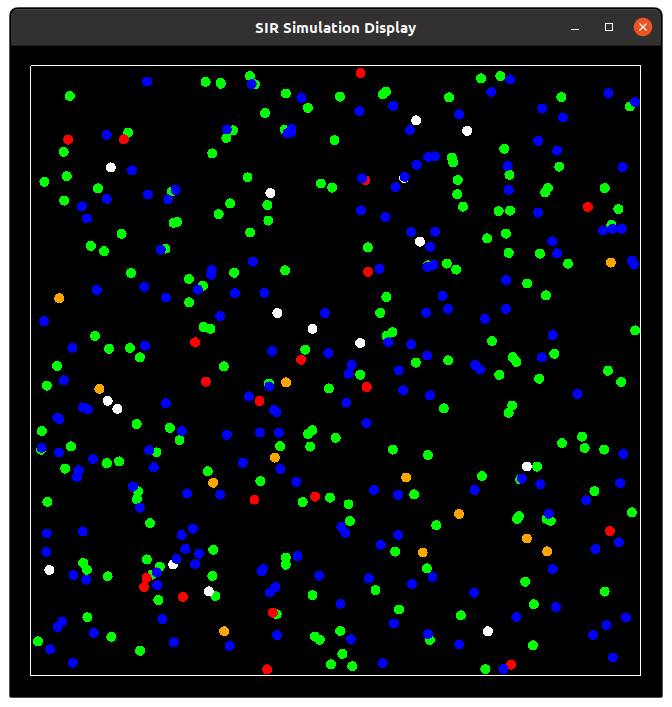
\includegraphics[width=\linewidth]{images/display.png}
    \caption{Finestra grafica ottenuta dalla classe Display. Il verde corrisponde ai sani, il rosso agli infettivi, l'arancione al virus in incubazione, il bianco alla quarantena e il blu ai guariti}
    \label{fig:display}
\end{figure}

Di seguito vengono riportati gli esiti di alcune simulazioni effettuate variando i parametri delle classi \emph{Infection} e \emph{Motion}. Se non diversamente indicato, i parametri  dello stato iniziale sono size = 600, S = 400, I = 10 e  R = 0. Si è scelto di iniziare la simulazione con 10 individui infettivi per velocizzarne l'esecuzione. Inoltre si è notato che  con un solo infetto può capitare che questo guarisca prima di infettare altre persone. Quest'ultimo caso, sebbene possibile, è stato ritenuto di scarso interesse.

La classe \emph{Motion} è stata inizializzata con una deviazione standard pari a 0.2. Si è notato che variare questo parametro influisce poco sulla simulazione. L'unica differenza apprezzabile è nella durata dell'epidemia, che diminuisce all'aumentare della varianza.

La classe \emph{Simple Infection} è stata inizializzata con una distanza critica di 10, una probabilità di infezione di 0.05 e un tempo di recupero di media 200 e deviazione standard 50. Inoltre, alla variante \emph{Incubation Infection}, si sono assegnati un tempo di incubazione di 50 e una probabilità di essere costretti alla quarantena di 0.005.

L'esito di una simulazione con i parametri sopra descritti e la classe \emph{Simple Infection} a gestire l'infezione è riportato in fig. \ref{fig:simple_005}. In fig. \ref{fig:simple_008} si può vedere come aumentando la probabilità di infezione a 0.08 il picco si alzi sensibilmente. Diminuire la size da 600 a 400, come mostrato in fig- \ref{fig:simple_400}, determina un'epidemia molto più violenta, con un picco alto e la totalità della popolazione che contrae il virus. Aumentarla a 800 (fig. \ref{fig:simple_800}), simulando una sorta di distanziamento sociale, provoca invece l'effetto opposto. Introducendo un periodo di incubazione si ottiene il grafico in fig. \ref{fig:incubation_005}, in cui si può notare come l'intensità dell'epidemia sia più modesta. Infine, aggiungendo la possibilità di essere costretti alla quarantena, si ottiene il grafico in fig. \ref{fig:quarantine}, in cui il numero di infetti è costantemente sotto controllo e il numero finale di individui che non contraggono il virus consistente.

\begin{figure*}[p]
    \centering
    \subfloat[][Probabilità: 0.05\label{fig:simple_005}]{
        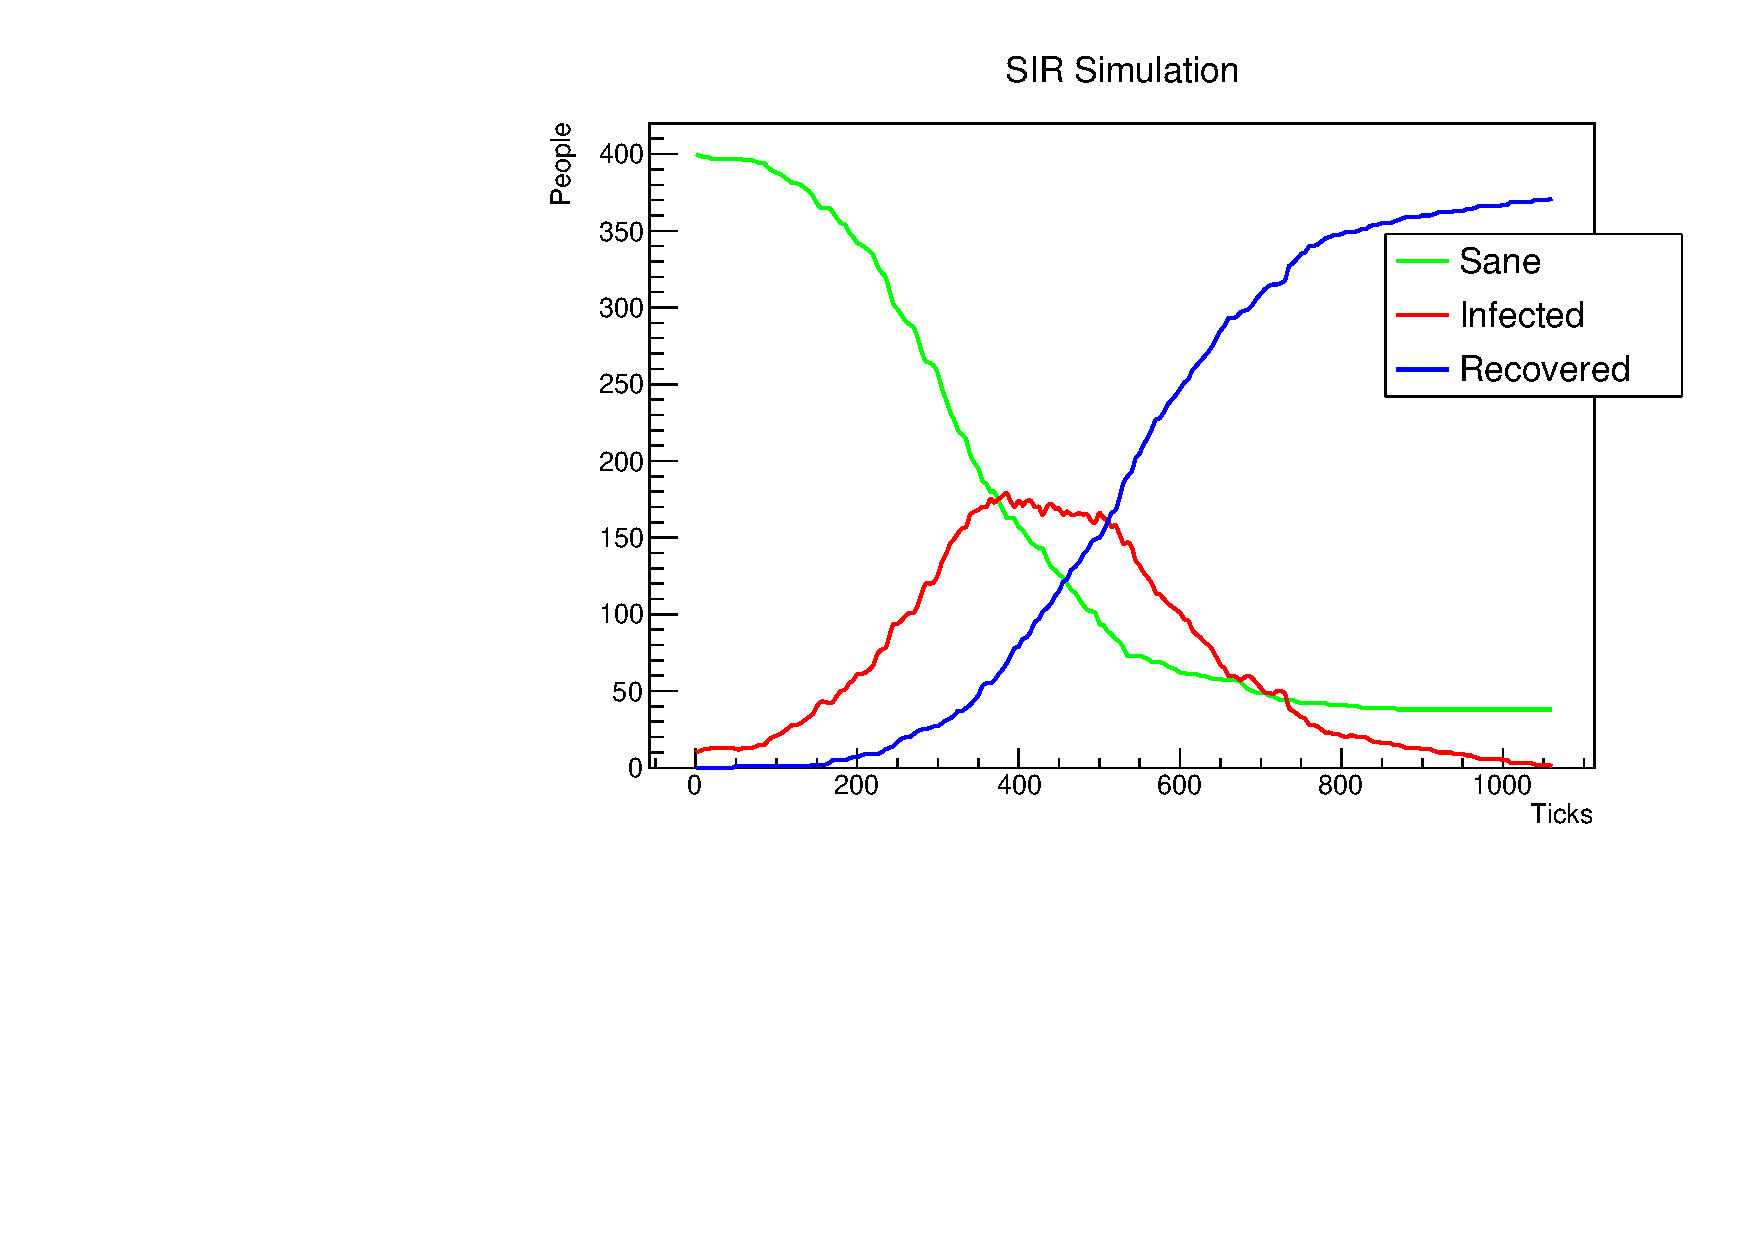
\includegraphics[width=0.5\textwidth]{images/simple_005.pdf}
    }
    \subfloat[][Probabilità: 0.08\label{fig:simple_008}]{
        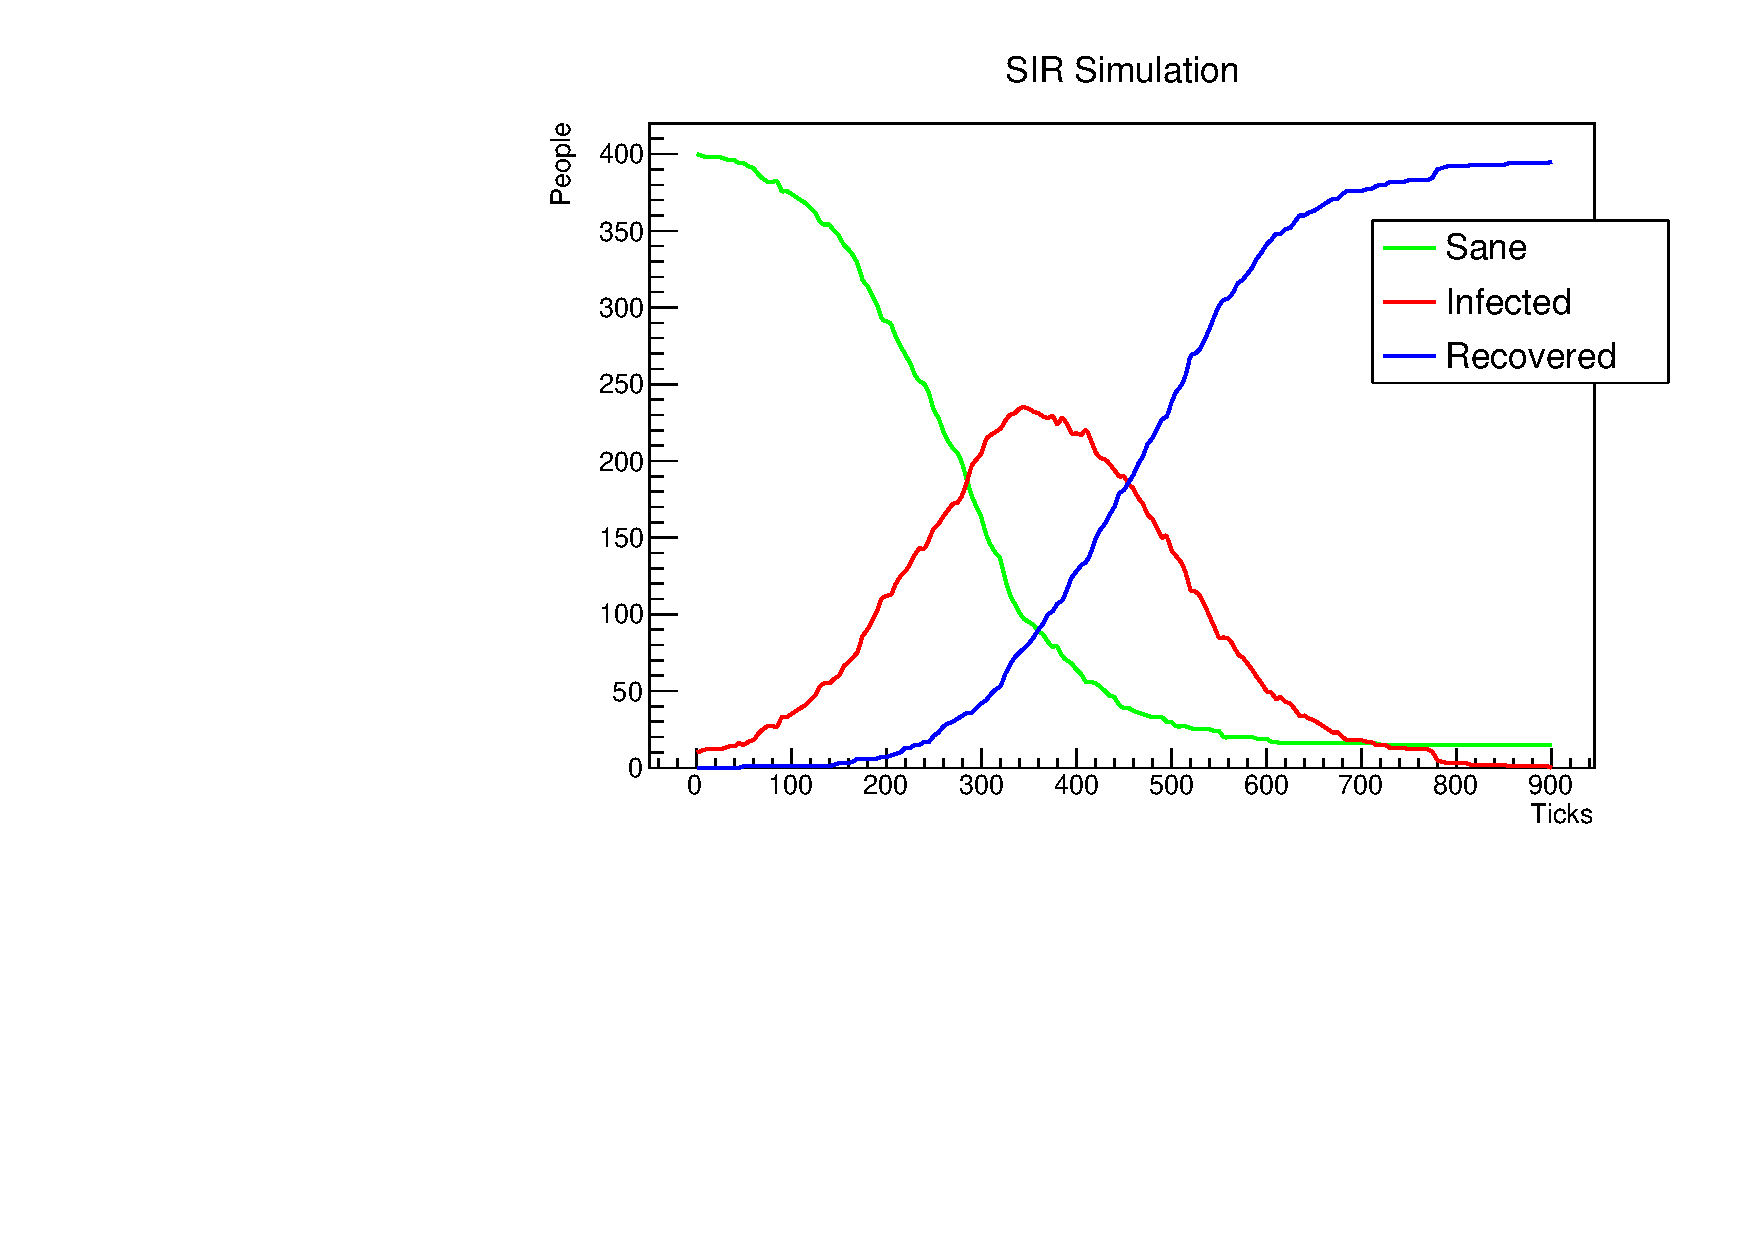
\includegraphics[width=0.5\textwidth]{images/simple_008.pdf}
    }
    \caption{Grafici di una simulazione con \emph{Simple Infection} a gestire l'infezione. I parametri della classe differiscono solo per la probabilità di infettarsi venendo a contatto con un indivuduo infettivo}
\end{figure*}

\begin{figure*}[p]
    \subfloat[][Size: 400\label{fig:simple_400}]{
        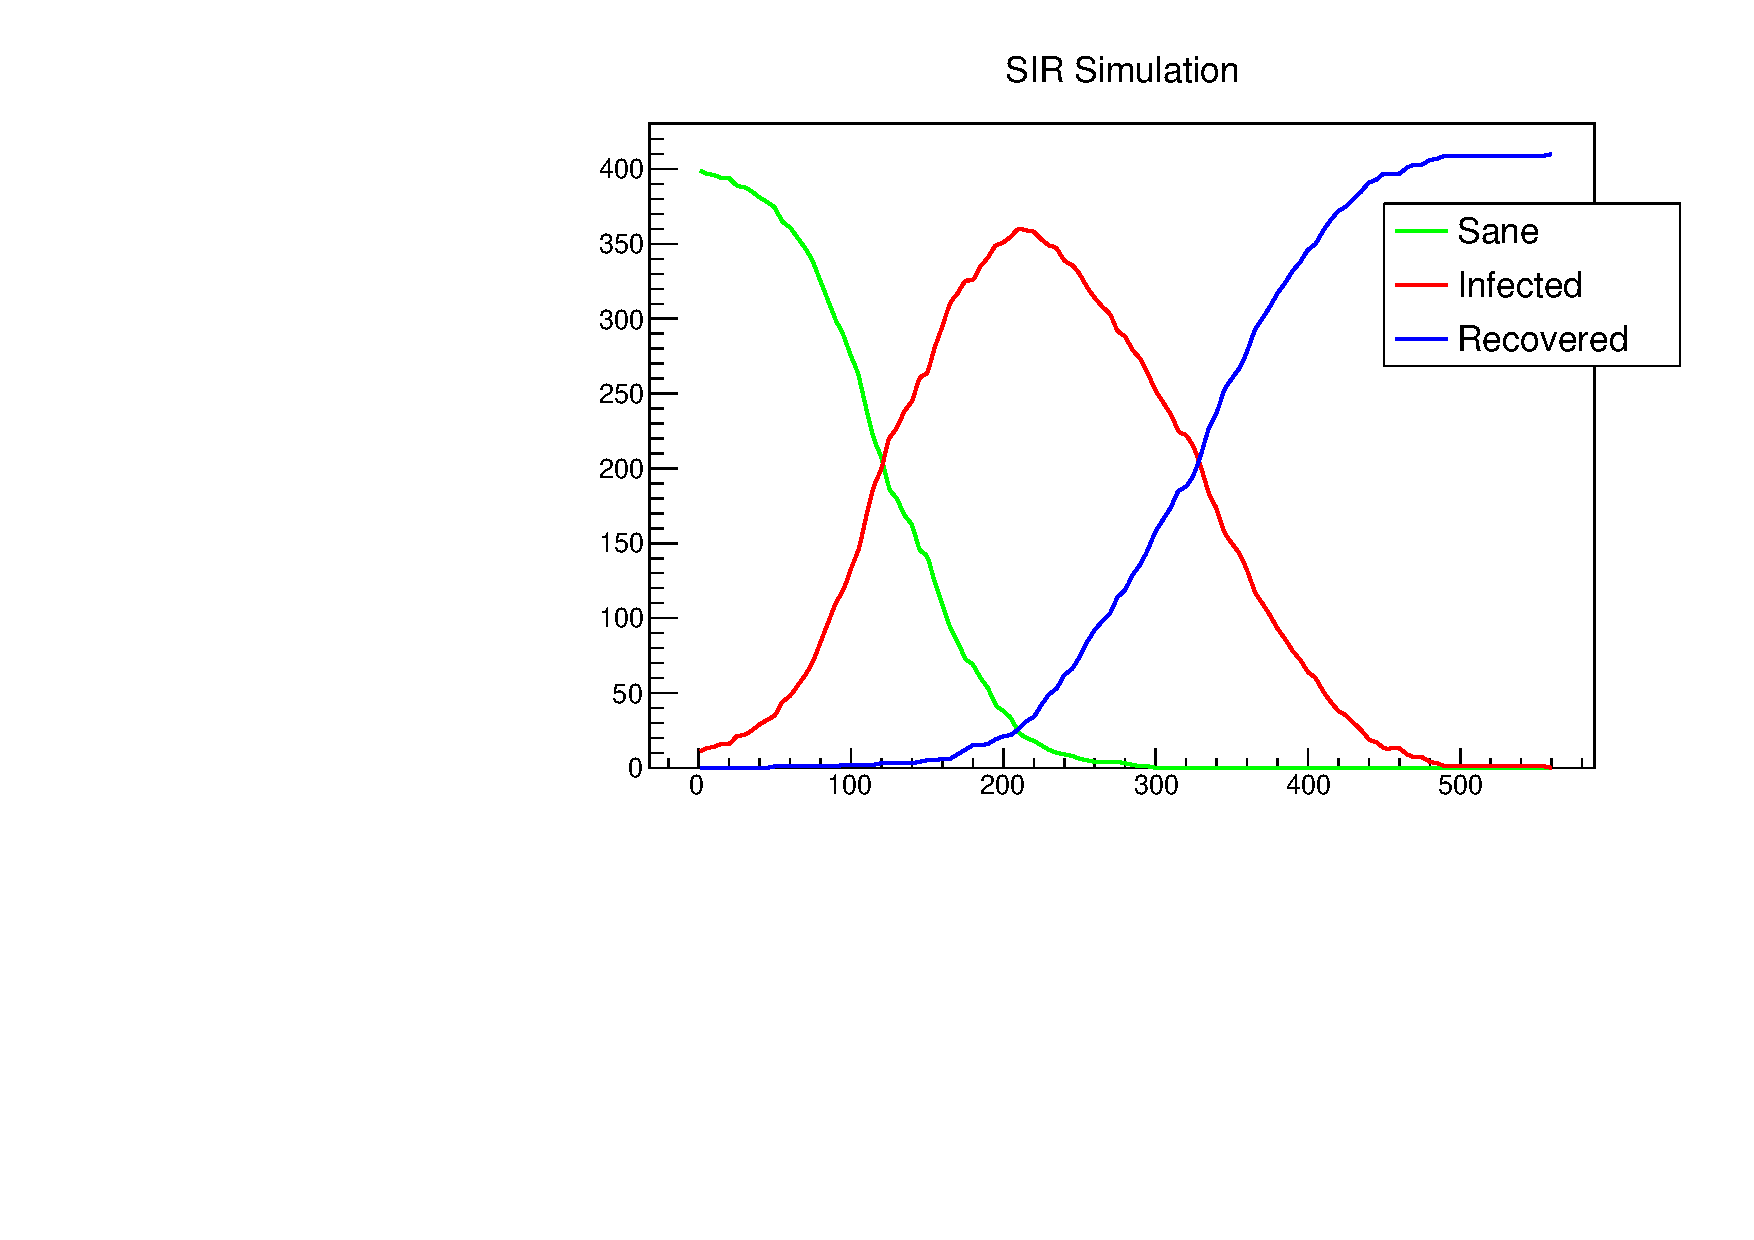
\includegraphics[width=0.5\textwidth]{images/simple_400.pdf}
    }
    \subfloat[][Size: 800\label{fig:simple_800}]{
        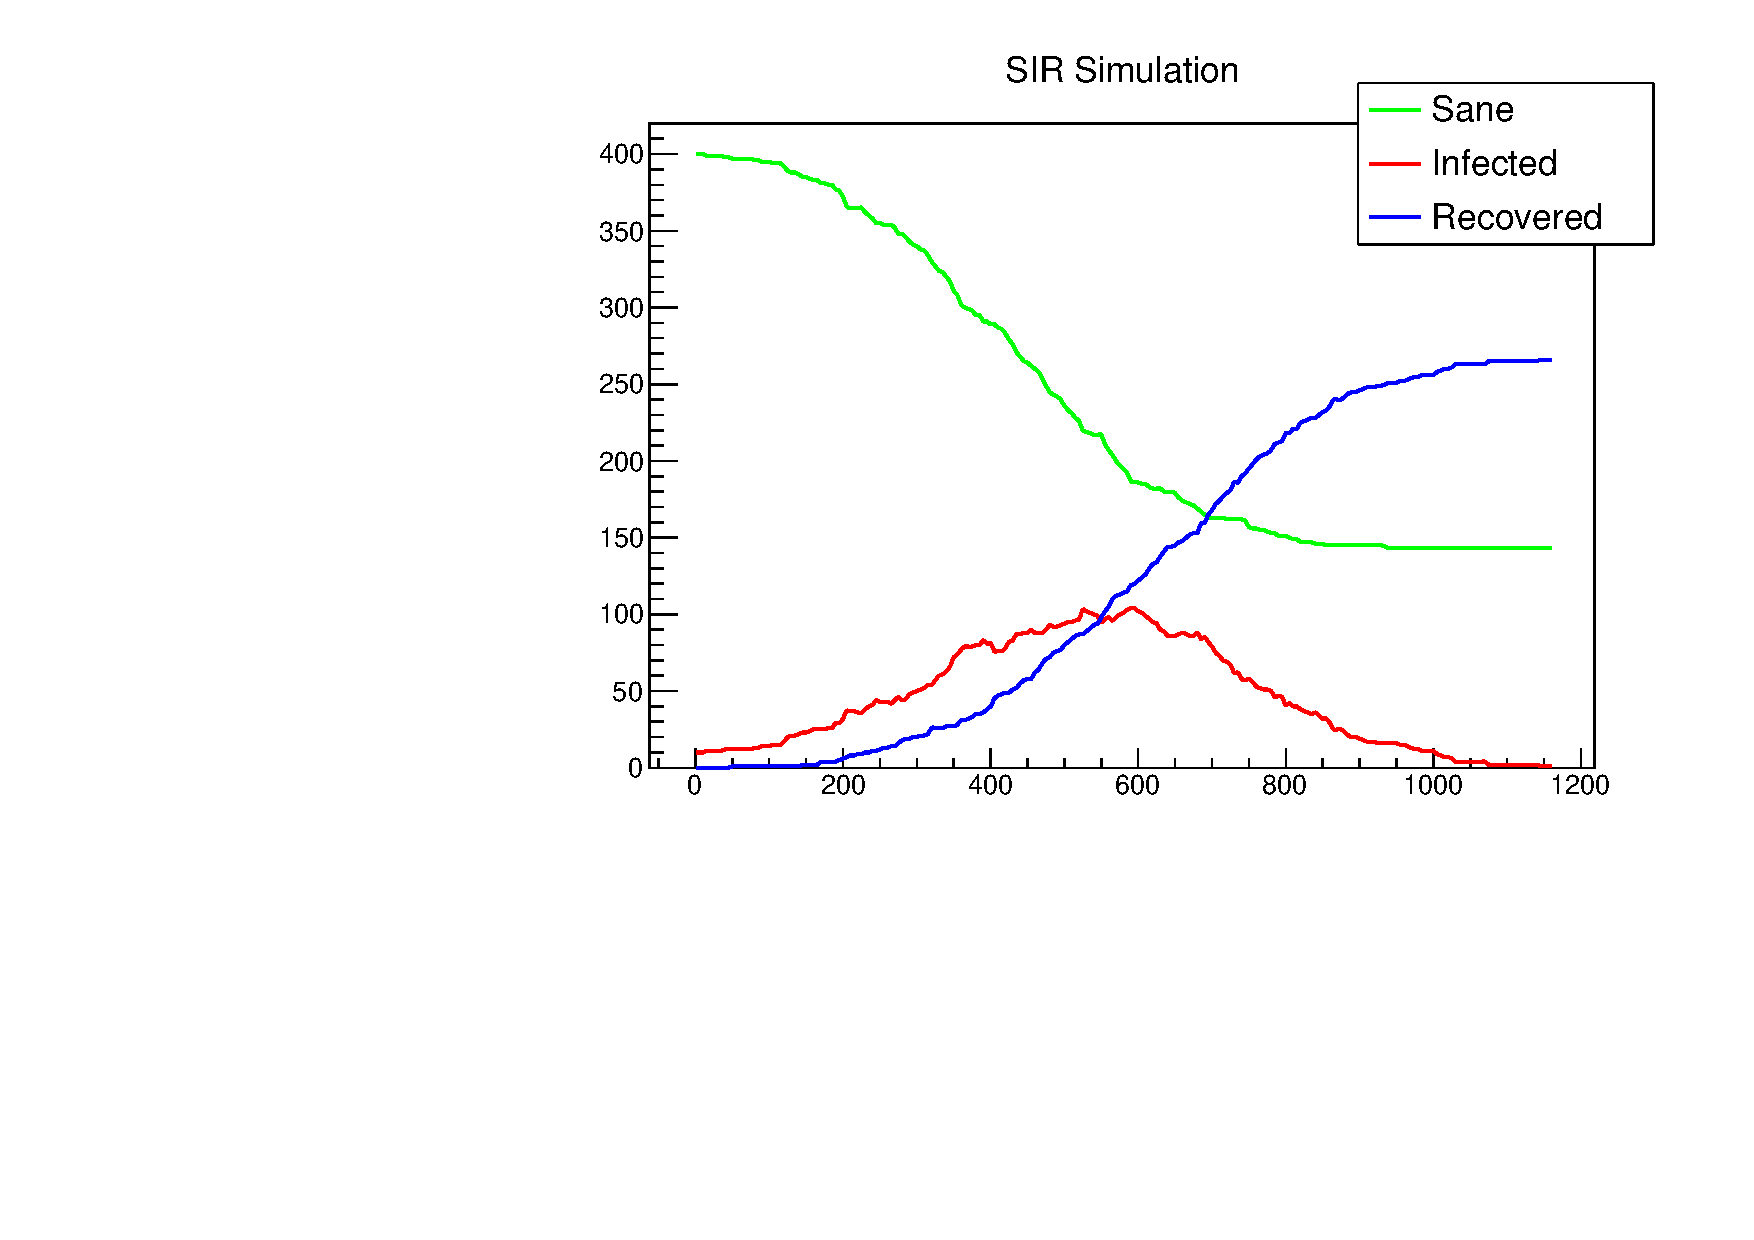
\includegraphics[width=0.5\textwidth]{images/simple_800.pdf}
    }
    \caption{Grafici di una simulazione con \emph{Simple Infection} a gestire l'infezione. I parametri della classe differiscono solo per la dimensione dello spazio a disposizione}
\end{figure*}

\begin{figure*}[p]
    \centering
    \subfloat[][Senza quarantena\label{fig:incubation_005}]{
        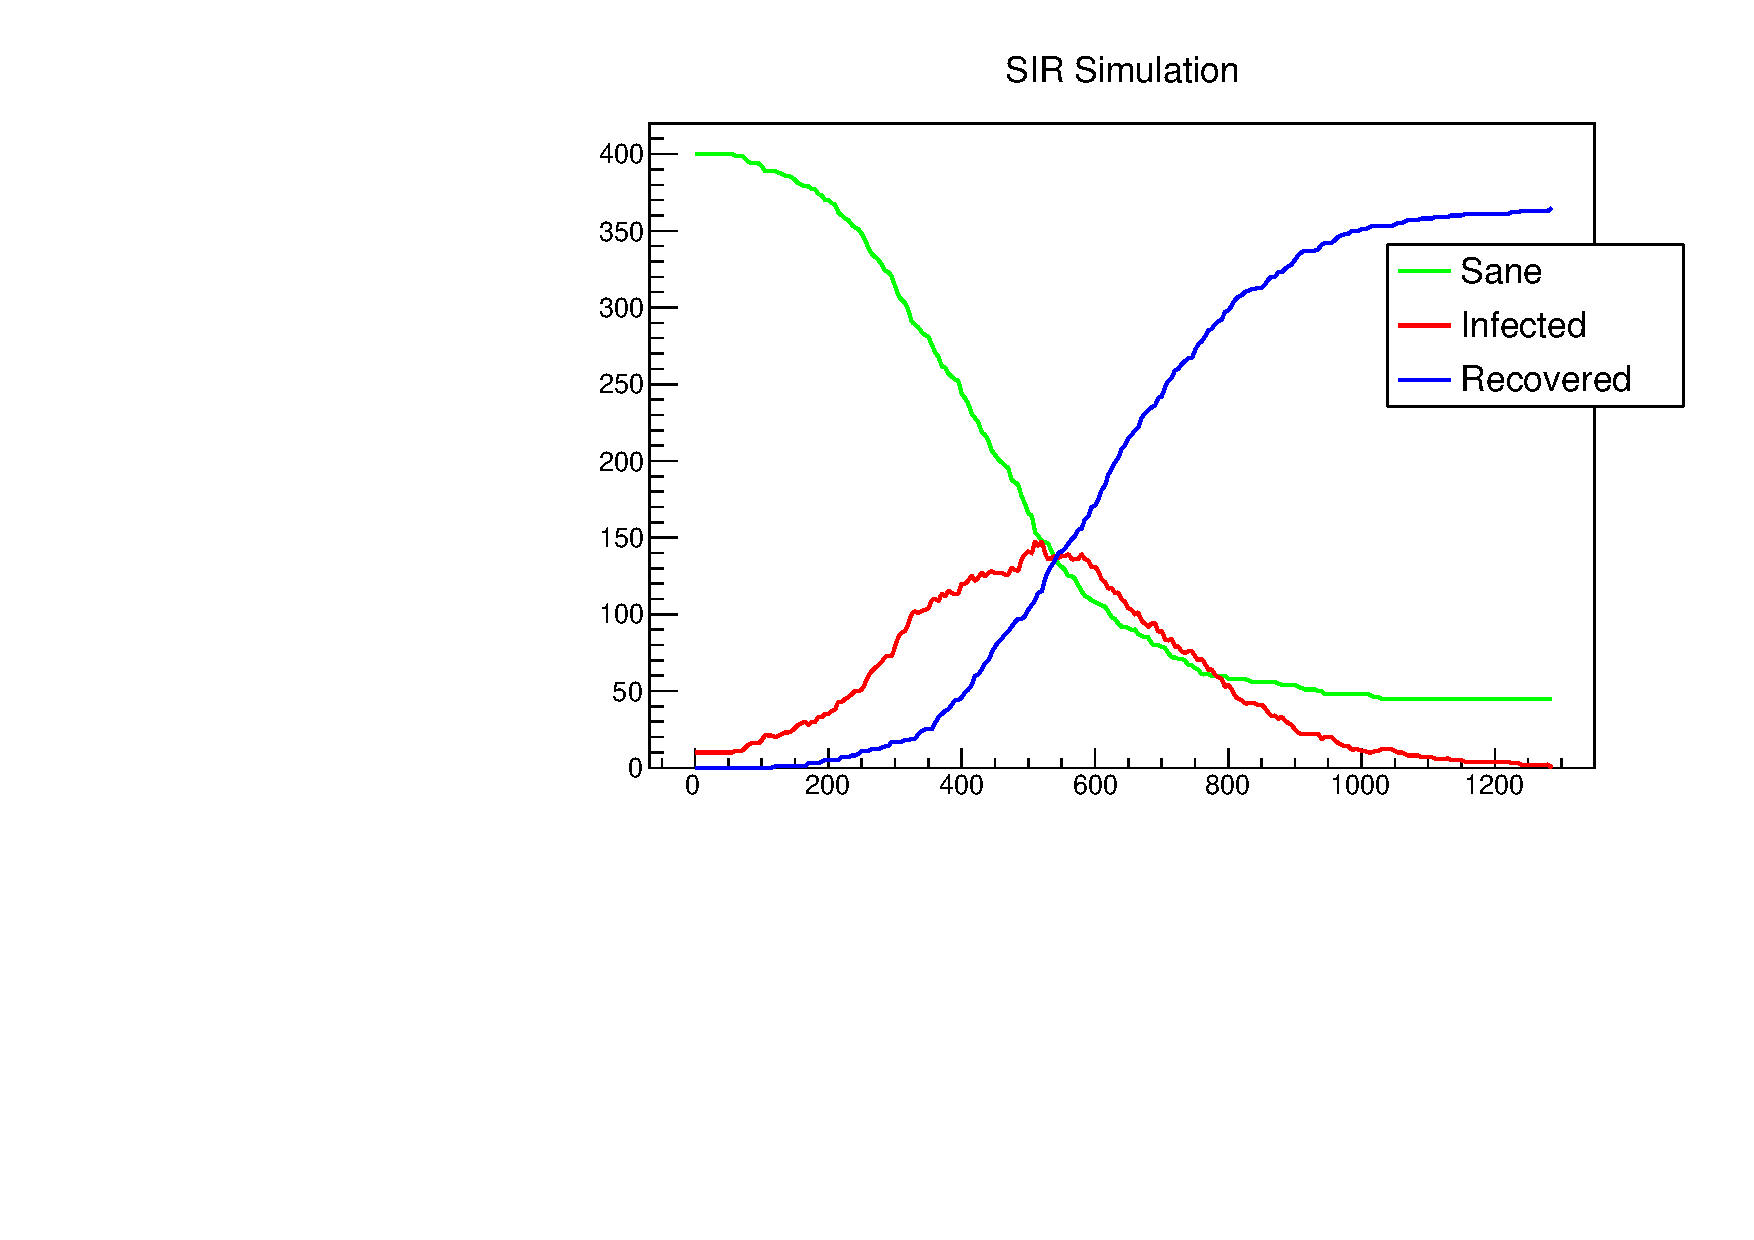
\includegraphics[width=0.5\textwidth]{images/incubation_005.pdf}
    }
    \subfloat[][Con quarantena\label{fig:quarantine}]{
        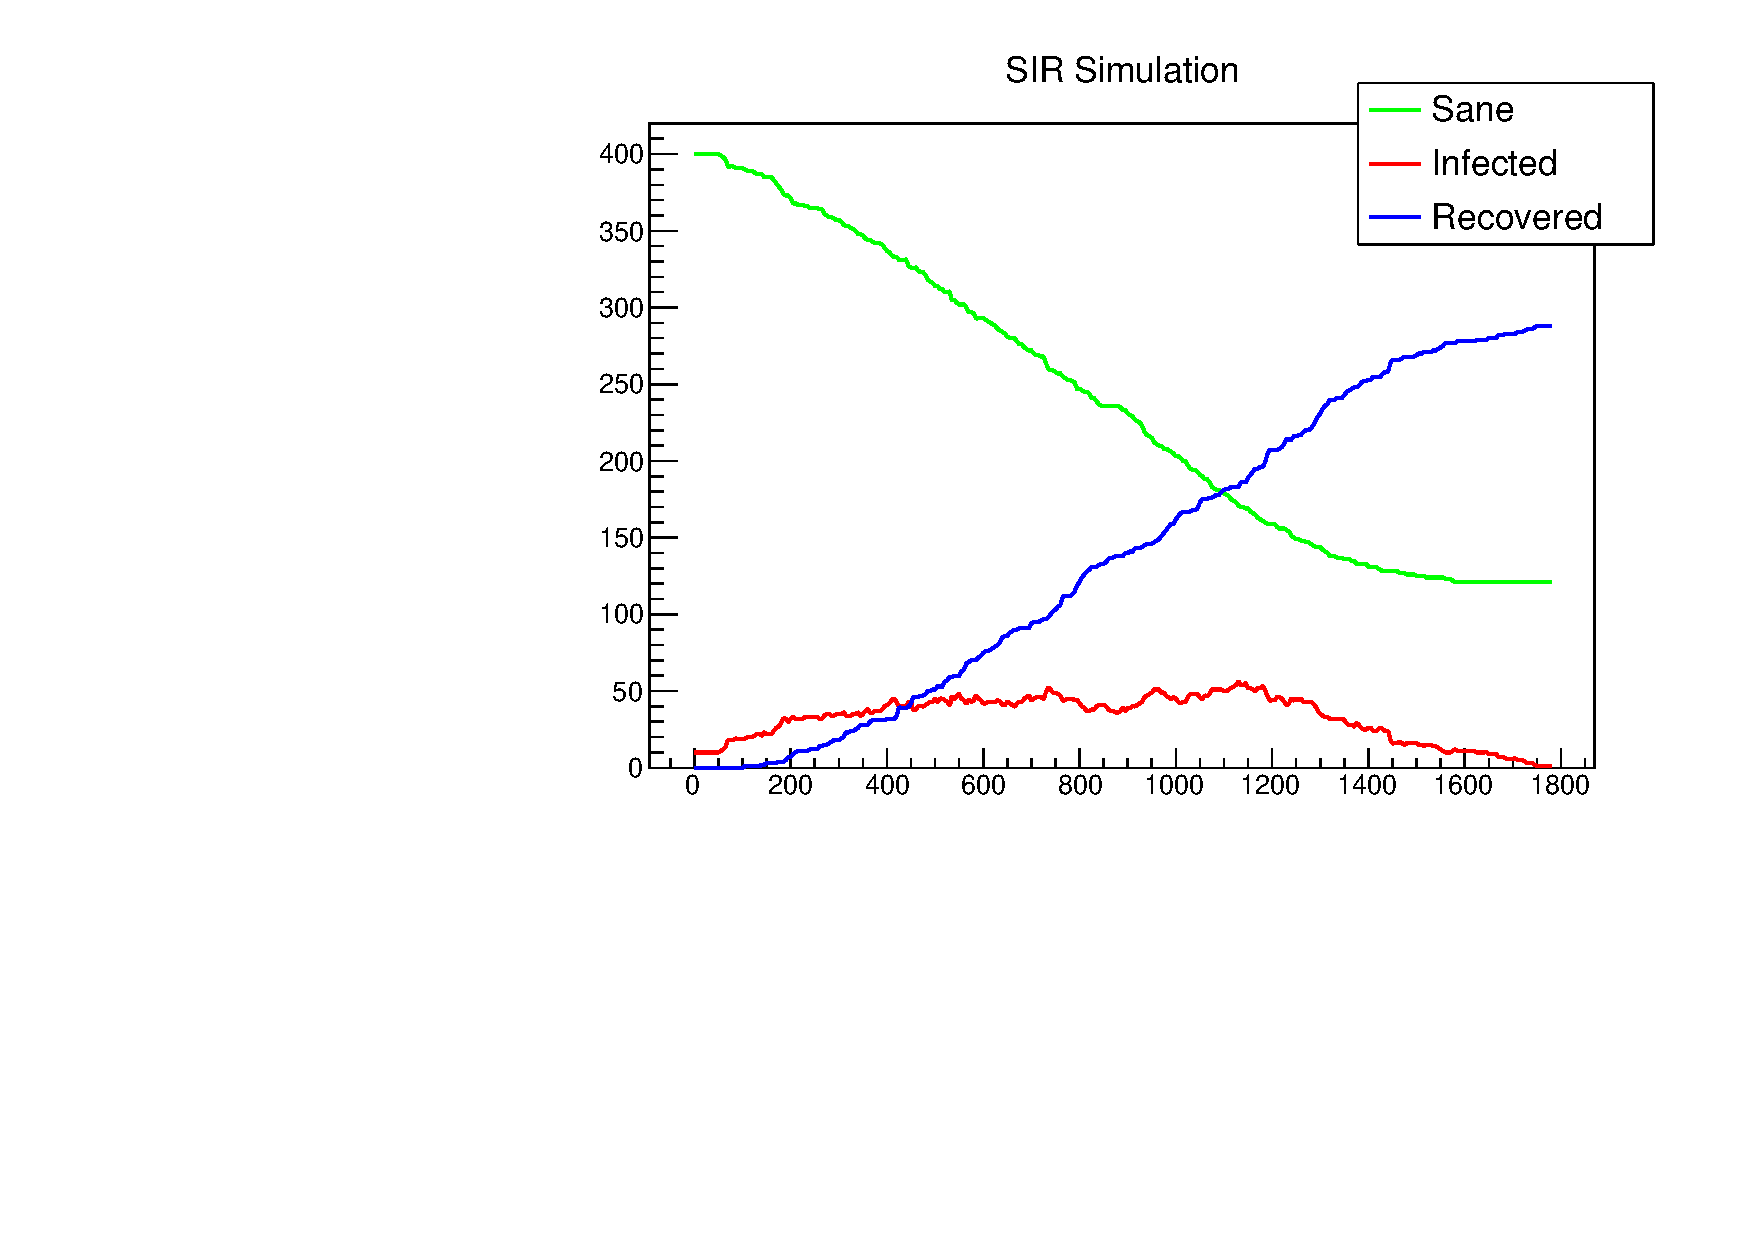
\includegraphics[width=0.5\textwidth]{images/quarantine.pdf}
    }
    \caption{Grafici di una simulazione con \emph{Incubation Infection} a gestire l'infezione. I parametri della classe sono gli stessi, ma nel secondo si è aggiunta la possibilità di essere costretti alla quarantena}
\end{figure*}

\section{Strategia di testing}
Per testare la correttezza del programma si è utilizzato \emph{Doctest}. Si è scelto di testare esplicitamente solo le classi \emph{Motion} e \emph{Infection}, dato che costituiscono il cuore del programma e sono le più suscettibili ad errori. Per le classi \emph{Display} e \emph{Plot}, che gestiscono l'output grafico, ci si è limitati a verificarne il corretto funzionamento durante l'esecuzione del programma.

\paragraph{Motion}
Per testare la classe \emph{Motion}, si è creata un'istanza con deviazione standard nulla, così da poter prevedere lo spostamento delle persone. Si è poi generata una popolazione di un solo individuo e si è verificato che la posizione venisse aggiornata correttamente, tenendo conto della velocità iniziale, della presenza dell'attrito e degli urti con le pareti. In seguito si è creata una seconda istanza di \emph{Motion} con deviazione standard non nulla e si è controllato che le medie delle posizioni, velocità e accelerazioni della popolazione fossero compatibili con una distribuzione delle accelerazioni di media zero.

\paragraph{Infection}
Le due classi che gestiscono l'infezione sono state testate con popolazioni ridotte, senza aggiornare la posizione degli individui. Gli individui sono stati distanziati in modo da poter prevedere i contatti e i parametri probabilistici delle classi sono stati impostati in modo da generare eventi certi o impossibili. Si è poi verificato che i contagi avvenissero come previsto, controllando sia la composizione dei vettori sia il \emph{Sub Status} degli individui.

\end{document}